\section{Interface interactive : dashboard Streamlit}
\label{sec:dashboard}

Afin de restituer les résultats de façon exploratoire, un \emph{dashboard}
\textbf{Streamlit} a été développé (dossier \texttt{dashboard/}). Il se lance
par la commande :
\begin{center}
\texttt{streamlit run dashboard/app.py}
\end{center}
et lit directement les sorties des scripts R/Python
(\texttt{results/figures/}, \texttt{results/tables/} et
\texttt{results/forecasts/}). Il est composé d'une page d'accueil et de cinq
pages accessibles via la barre latérale. Les captures d'écran ci-dessous
(documentées dans \texttt{results/dashboard/}) illustrent chaque interface.

\subsection{Vue d'ensemble}
La page d'accueil affiche des indicateurs synthétiques (nombre de figures, de
tableaux et de prévisions) et le \emph{Top 8} des meilleurs RMSE par couple
(Variable, Horizon), extrait de \texttt{py\_evaluation\_ranking.csv}.

\begin{figure}[H]
\centering
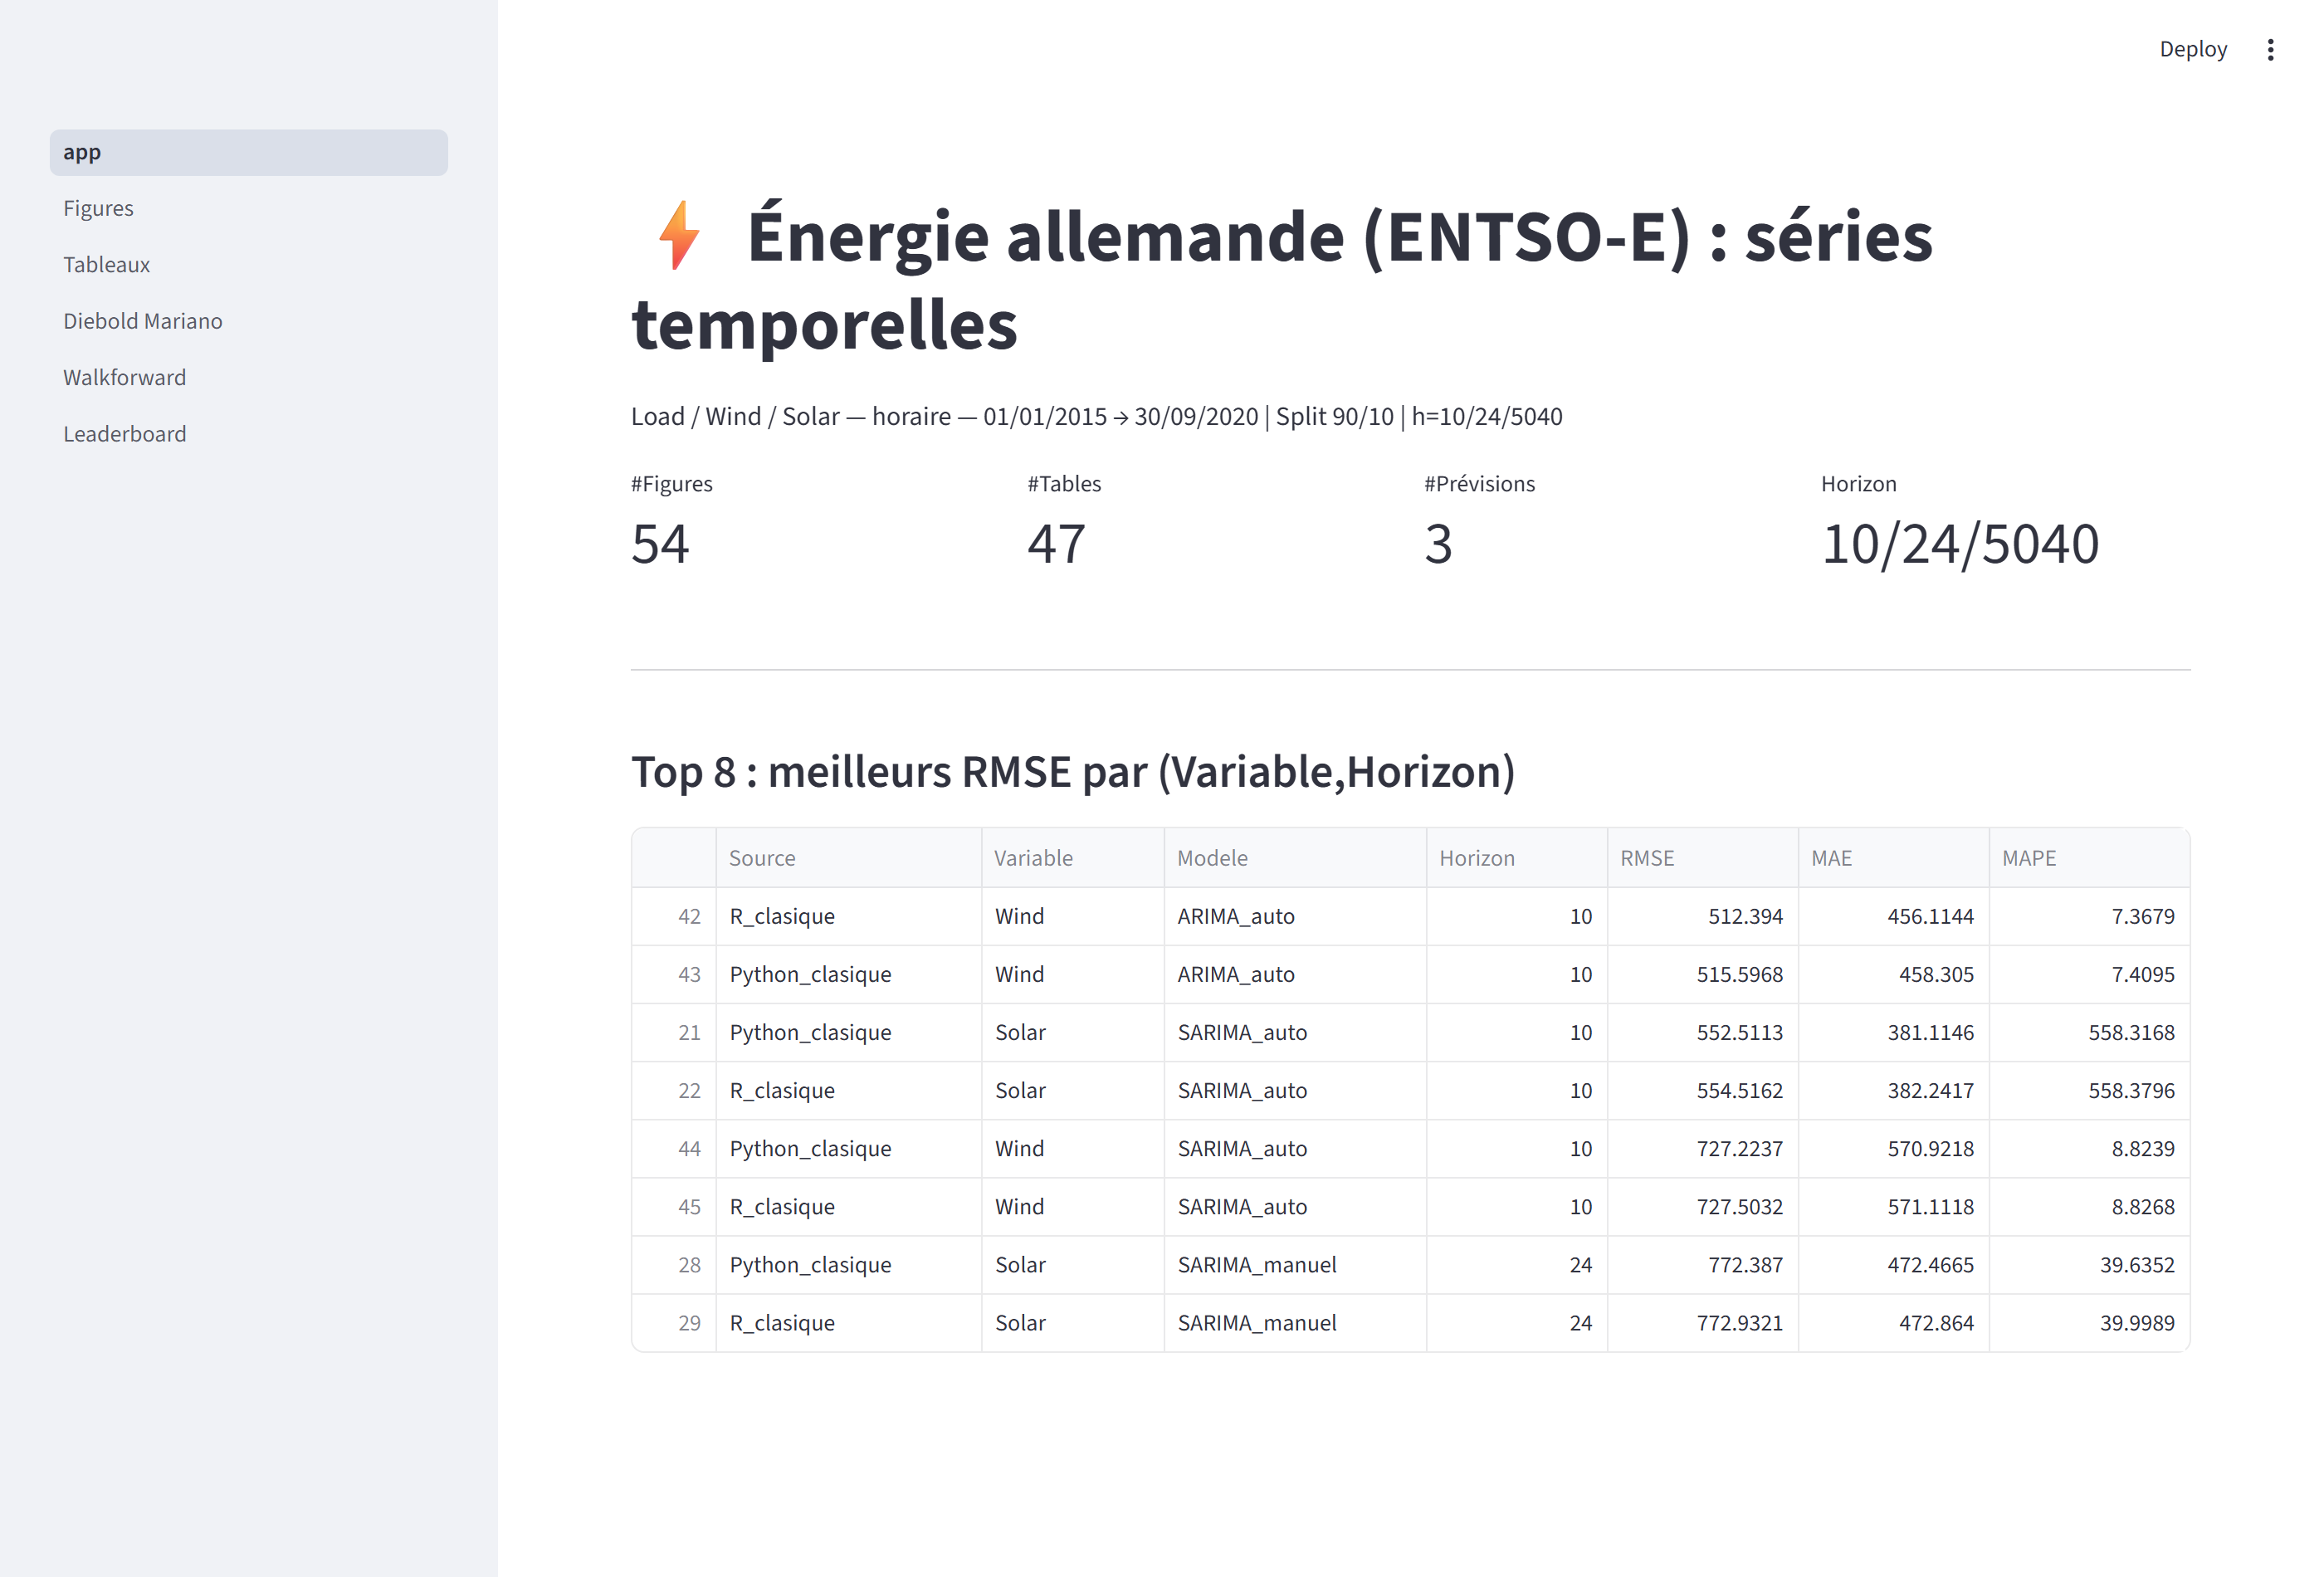
\includegraphics[width=0.9\textwidth]{dashboard_overview.png}
\caption{Interface Streamlit --- page « Vue d'ensemble ».}
\label{fig:dash_overview}
\end{figure}

\subsection{Page « Figures »}
Cette page constitue une galerie de l'ensemble des figures générées
(\(54\) fichiers \texttt{*.png}) avec leur légende.

\begin{figure}[H]
\centering
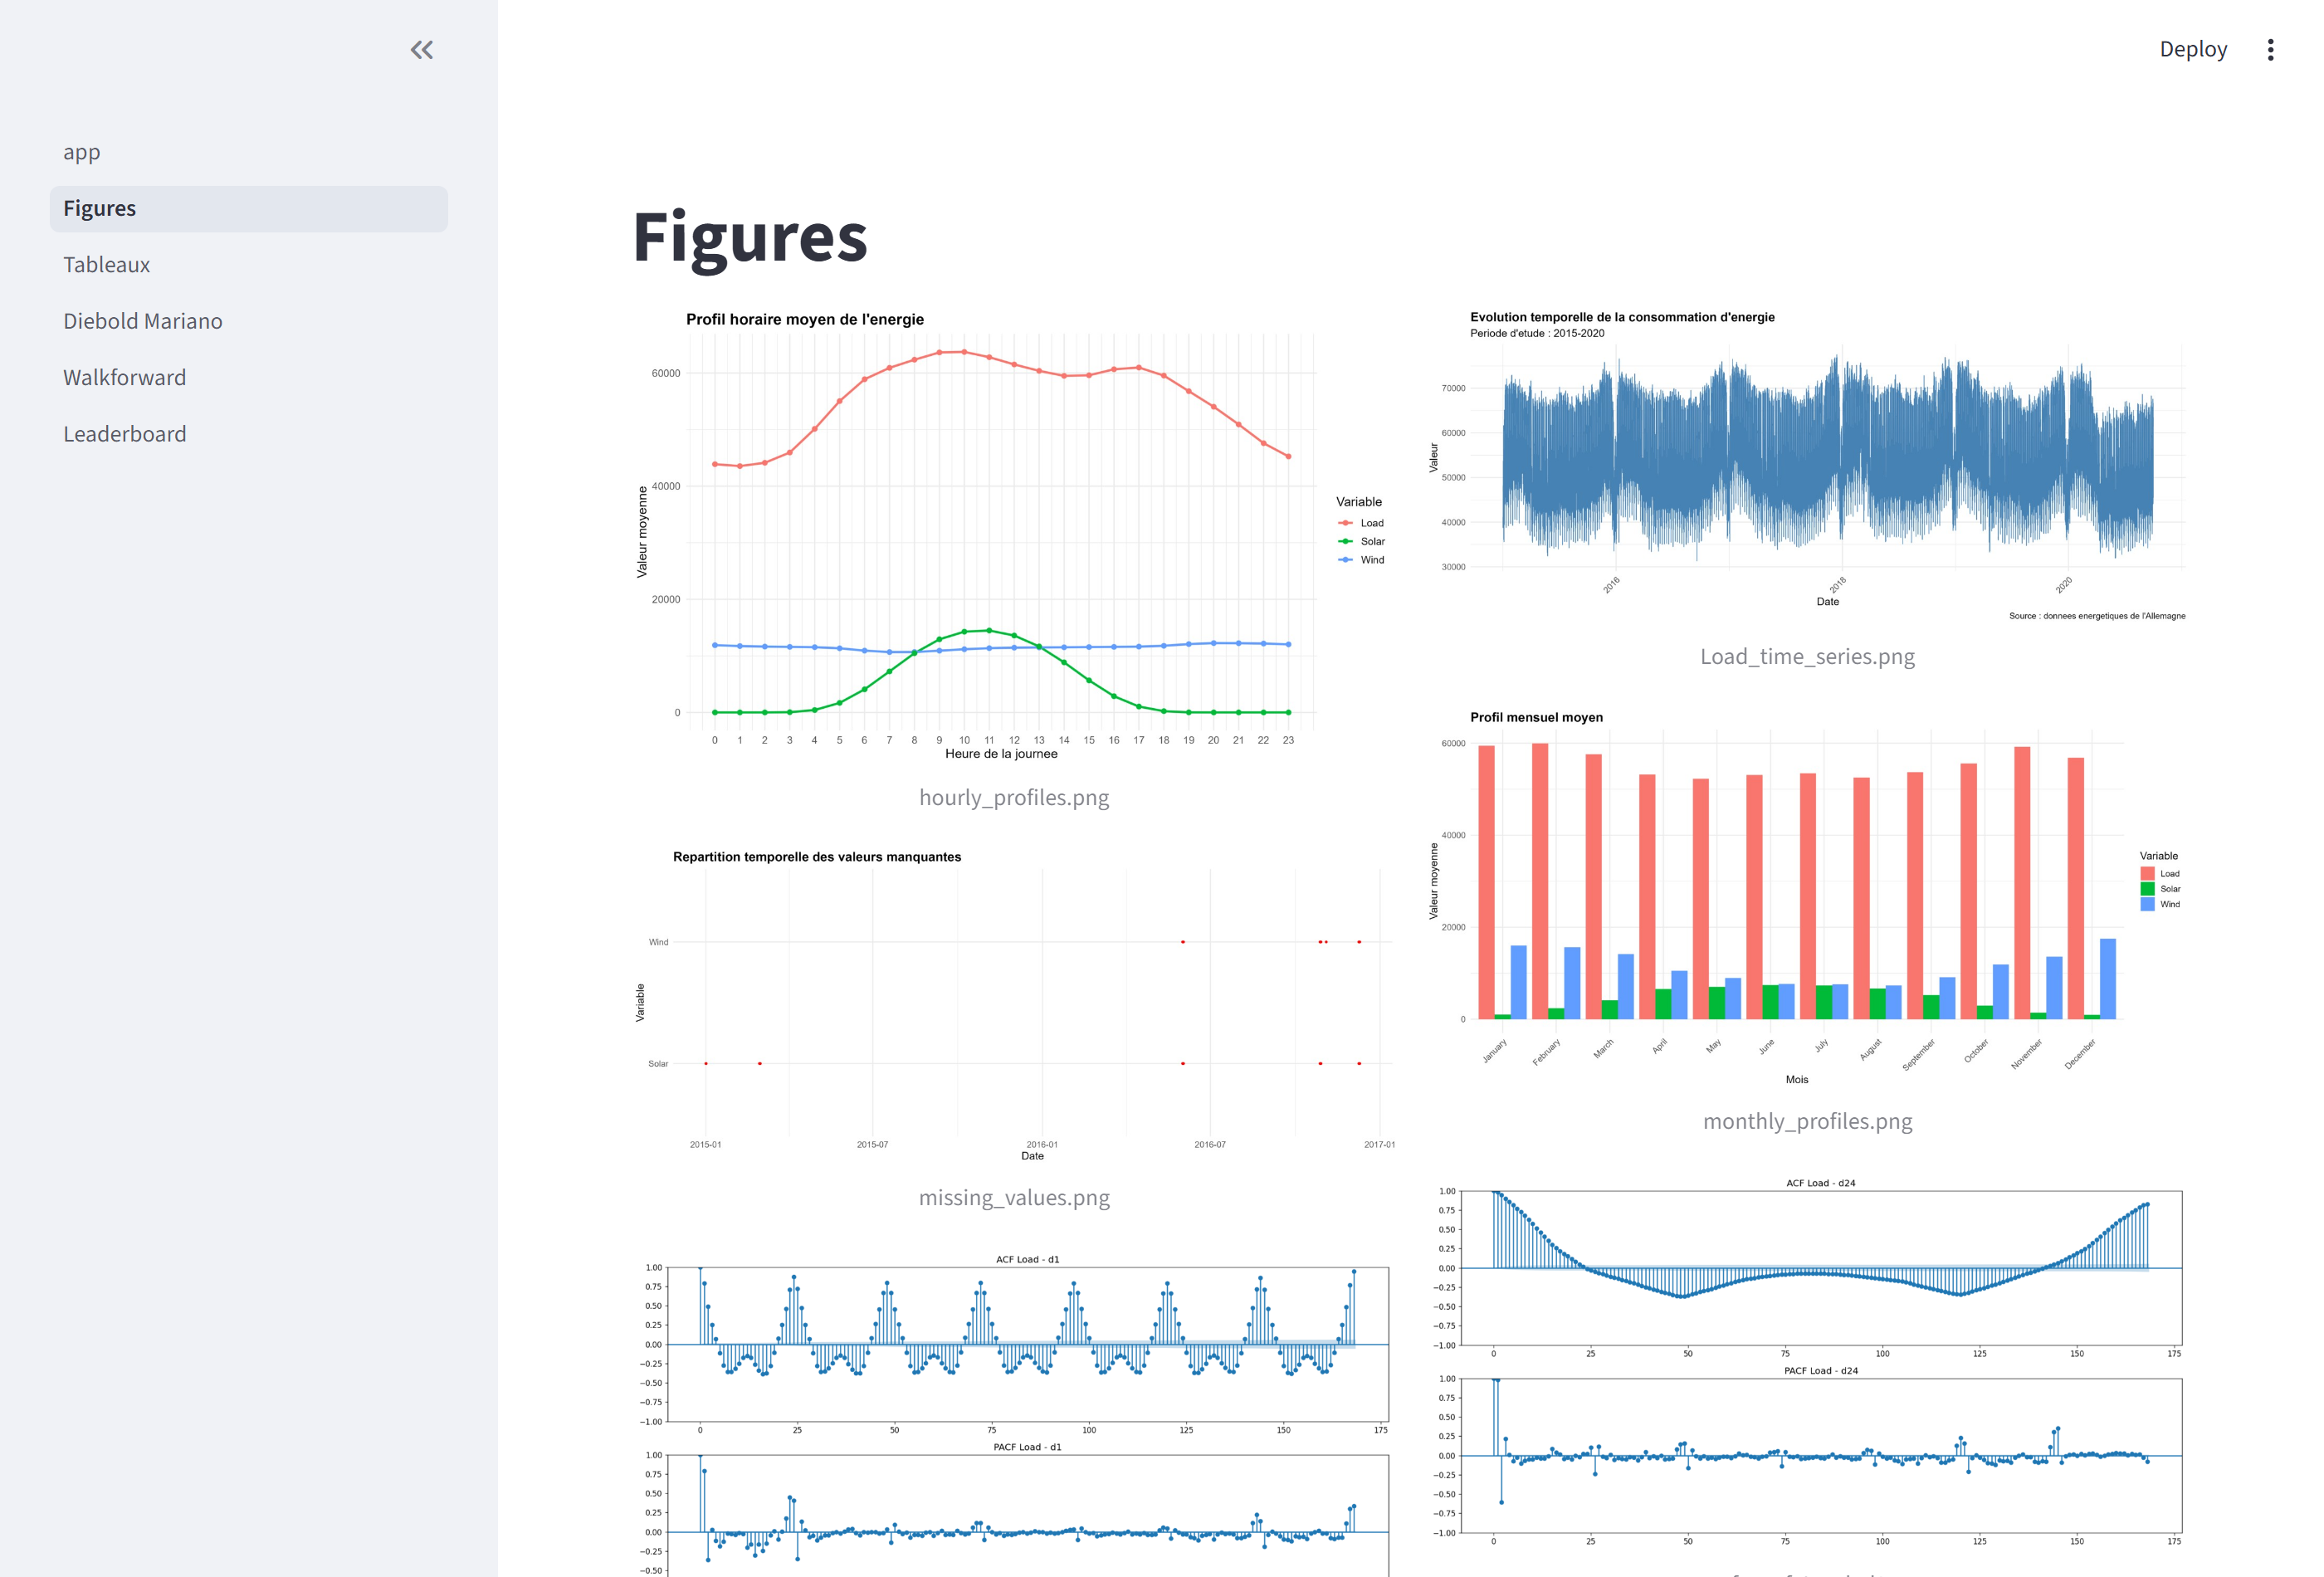
\includegraphics[width=0.9\textwidth]{dashboard_figures.png}
\caption{Interface Streamlit --- galerie « Figures ».}
\label{fig:dash_figures}
\end{figure}

\subsection{Page « Tableaux de résultats »}
Un sélecteur latéral permet de parcourir les \(47\) tables CSV produites, et
de visualiser n'importe quel tableau de résultats.

\begin{figure}[H]
\centering
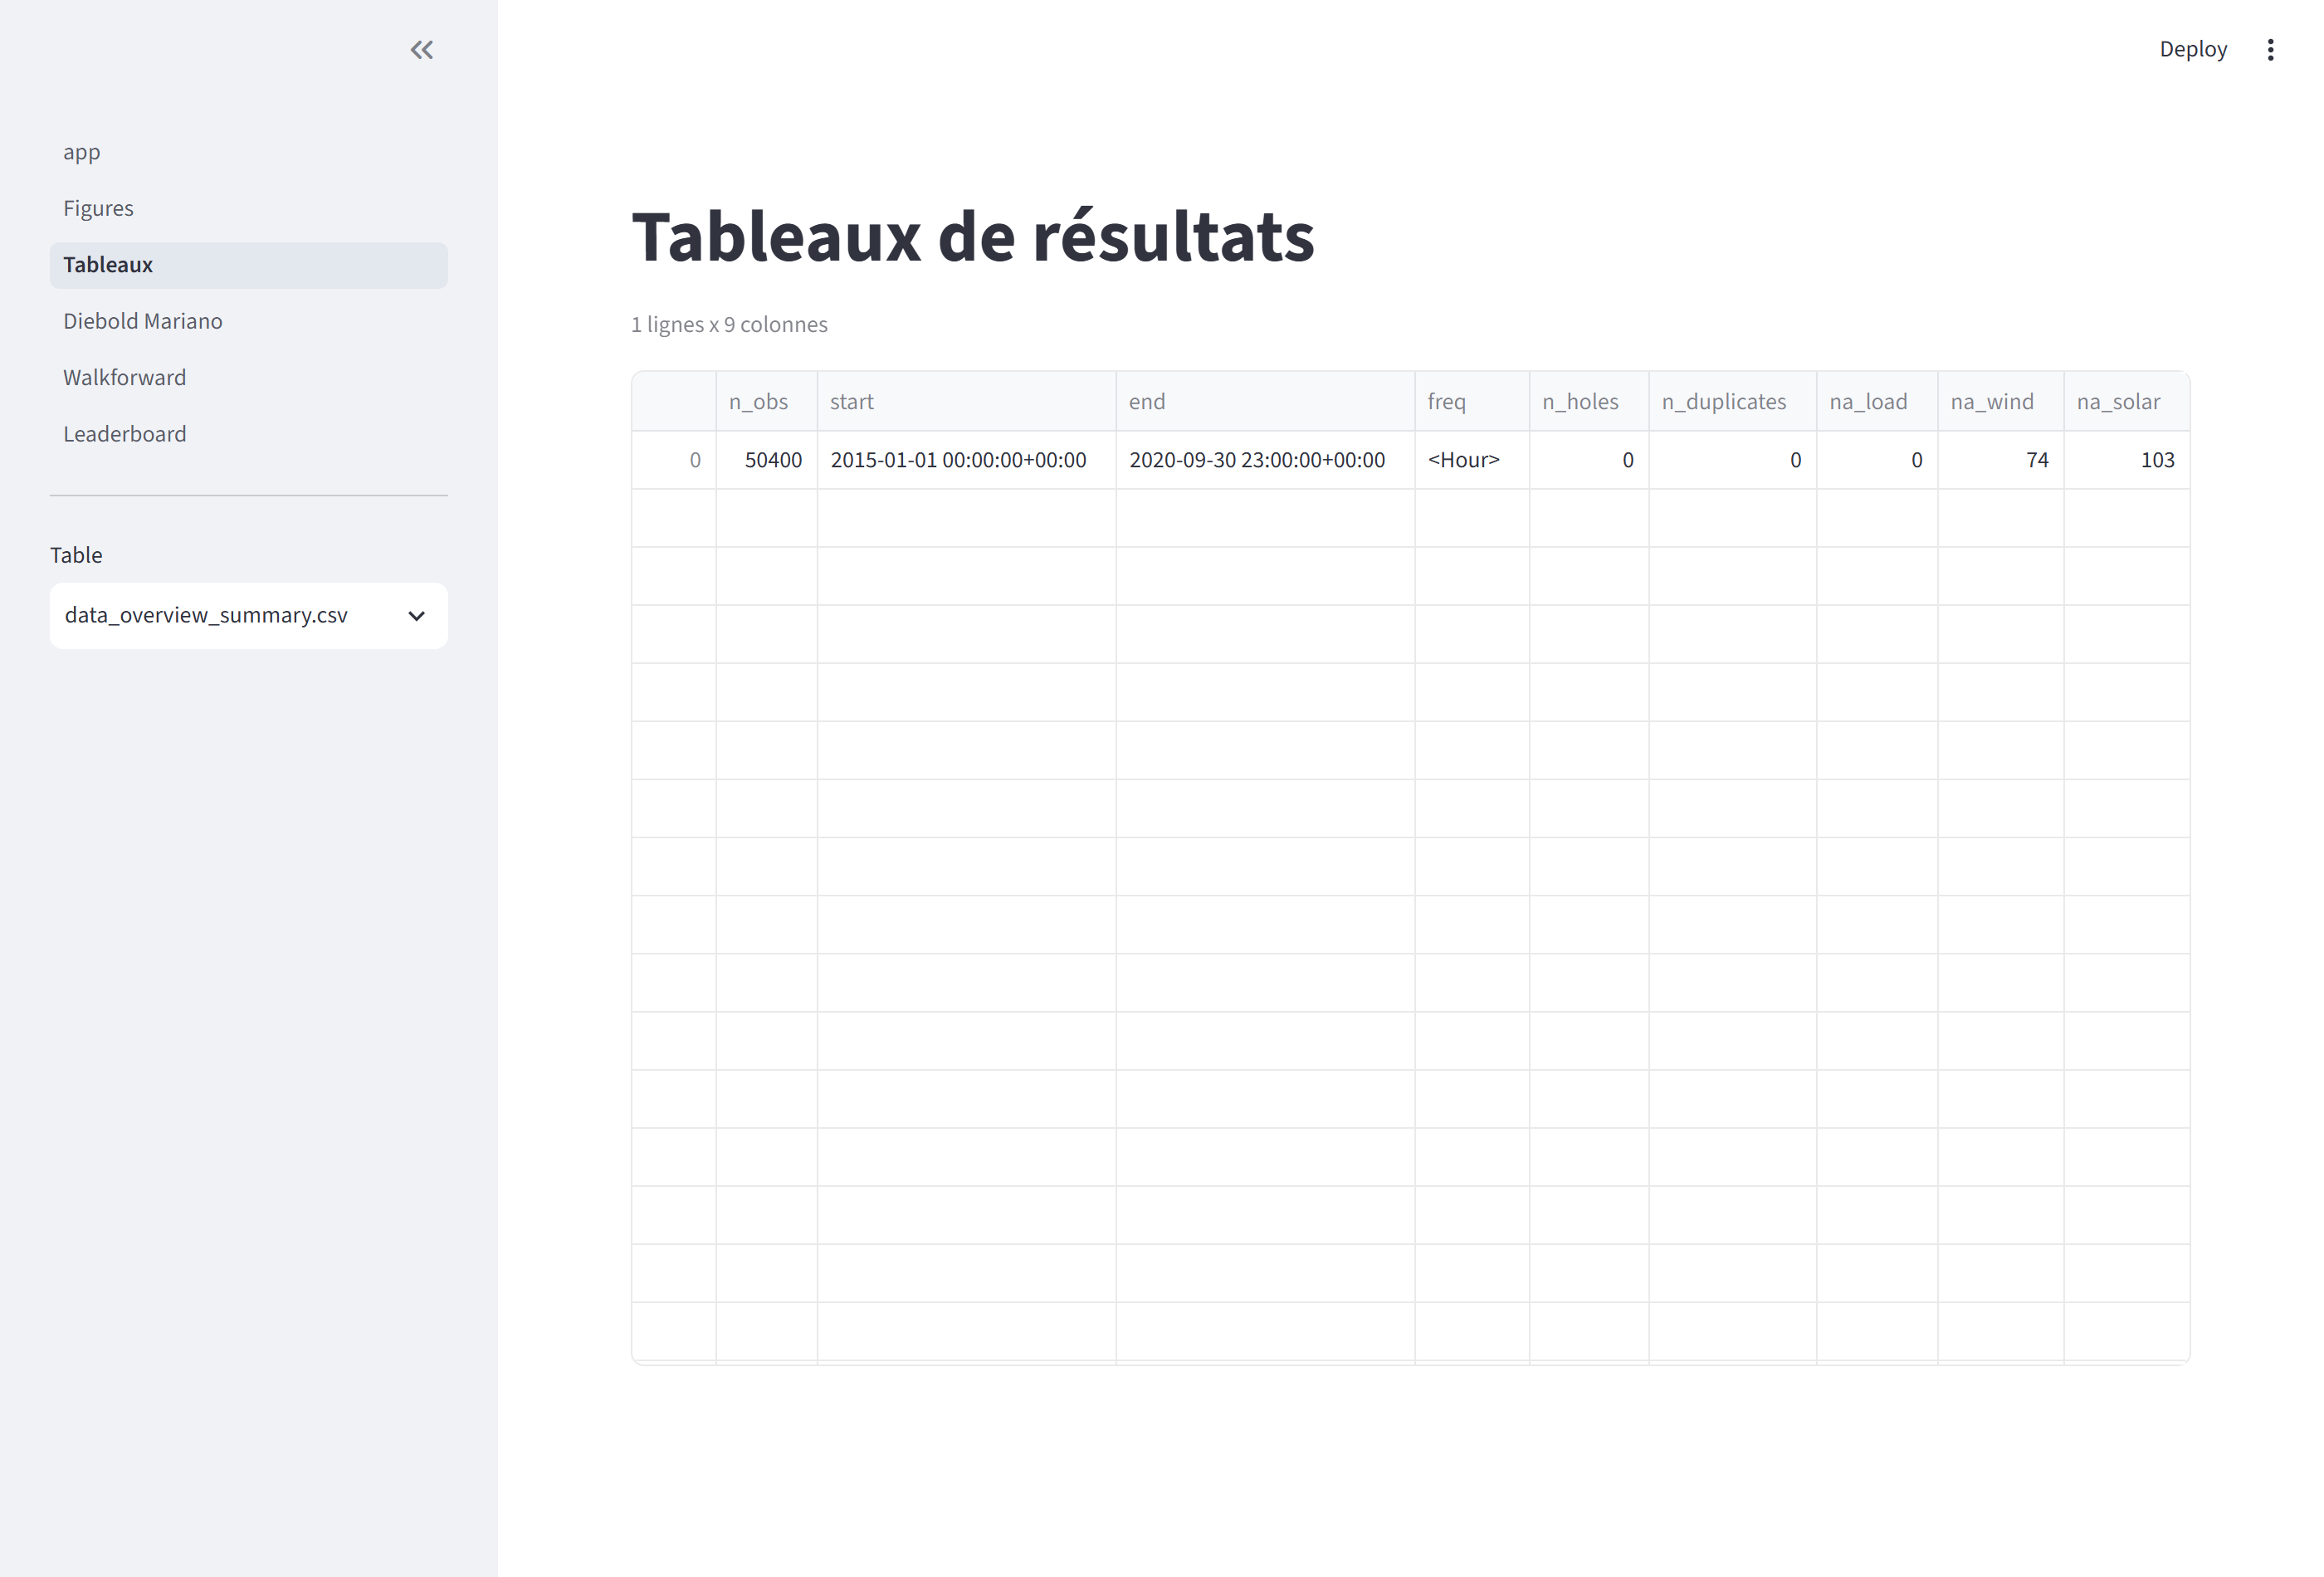
\includegraphics[width=0.9\textwidth]{dashboard_tableaux.png}
\caption{Interface Streamlit --- exploration des tableaux CSV.}
\label{fig:dash_tableaux}
\end{figure}

\subsection{Page « Diebold--Mariano »}
Cette page présente le tableau du test de Diebold--Mariano
(\texttt{py\_diebold\_mariano.csv}) comparant \textbf{toutes les paires} de
modèles du walk-forward (naïfs, SARIMA, LSTM, GRU).

\begin{figure}[H]
\centering
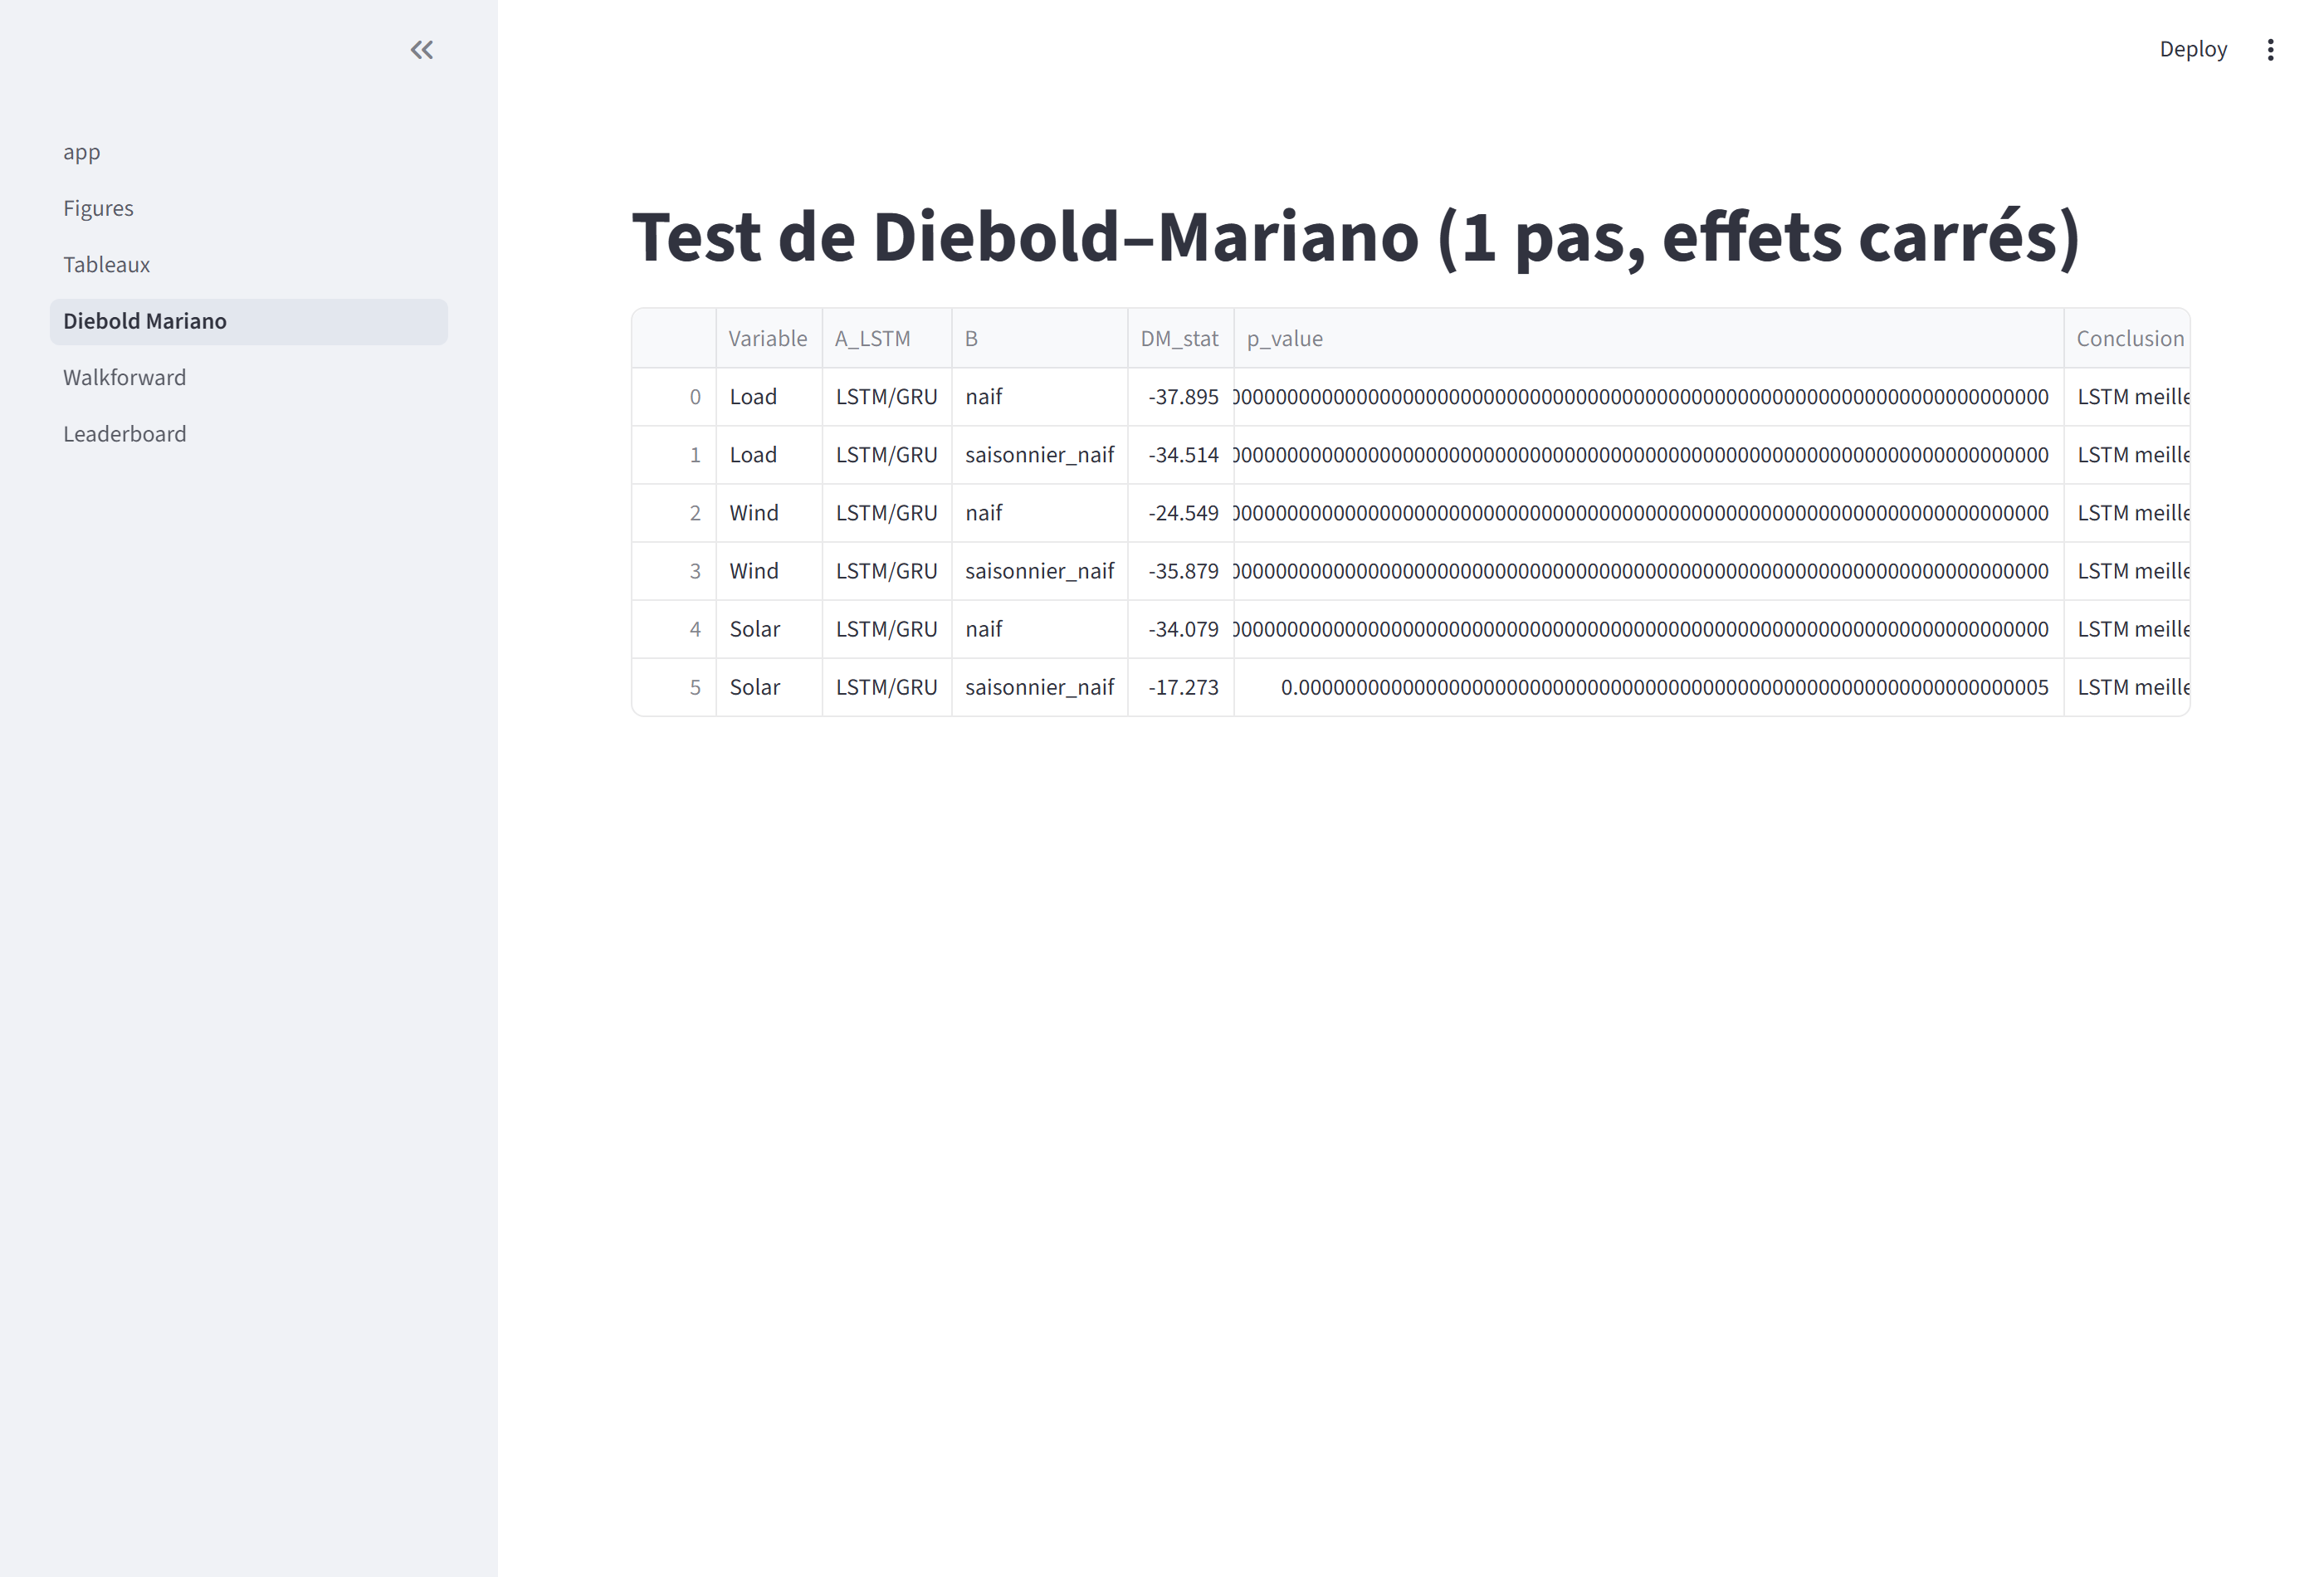
\includegraphics[width=0.9\textwidth]{dashboard_diebold_mariano.png}
\caption{Interface Streamlit --- test de Diebold--Mariano.}
\label{fig:dash_dm}
\end{figure}

\subsection{Page « Prévisions walk-forward »}
Un graphique interactif (Plotly) permet de sélectionner une variable et de
comparer la série observée aux prévisions à un pas (SARIMA, LSTM, GRU, naïf,
saisonnier naïf), avec une vue zoomée sur les 200 premiers points.

\begin{figure}[H]
\centering
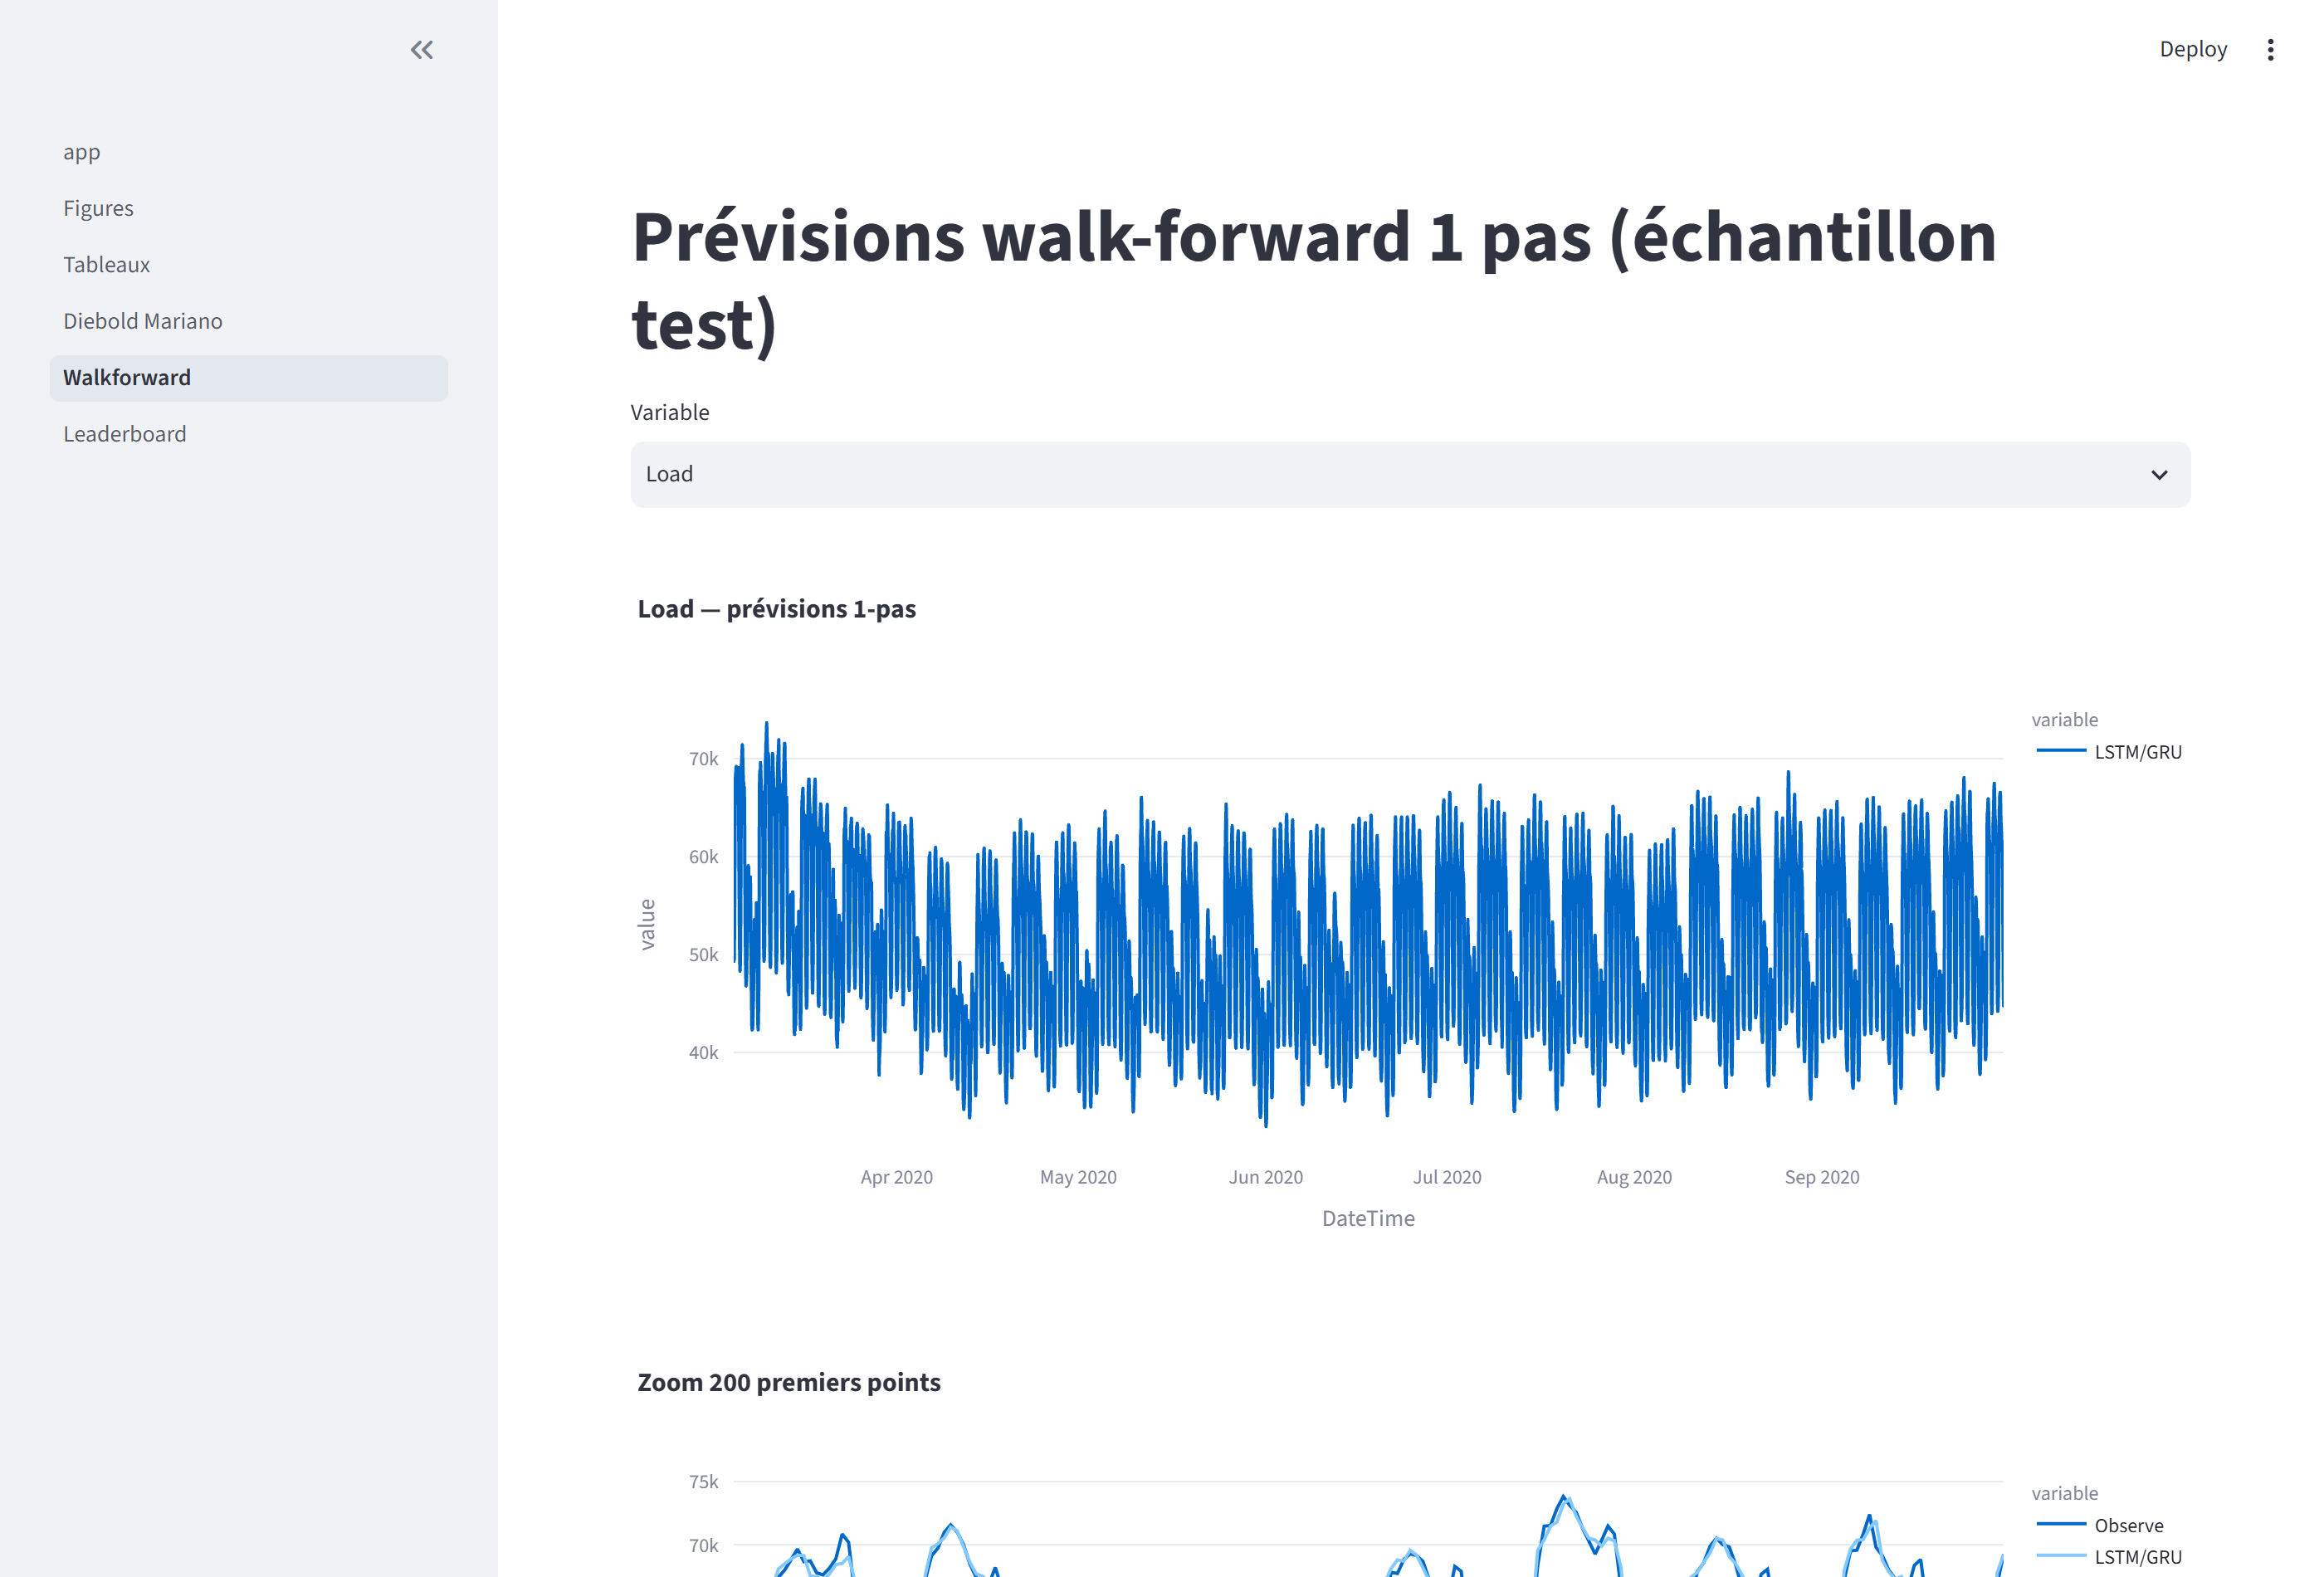
\includegraphics[width=0.9\textwidth]{dashboard_walkforward.png}
\caption{Interface Streamlit --- prévisions walk-forward.}
\label{fig:dash_wf}
\end{figure}

\subsection{Page « Leaderboard »}
Enfin, cette page classe par RMSE les modèles (R, Python classique, LSTM/GRU,
Prophet, hybride) pour une variable et un horizon choisis, sous forme de
tableau et de diagramme en barres interactif.

\begin{figure}[H]
\centering
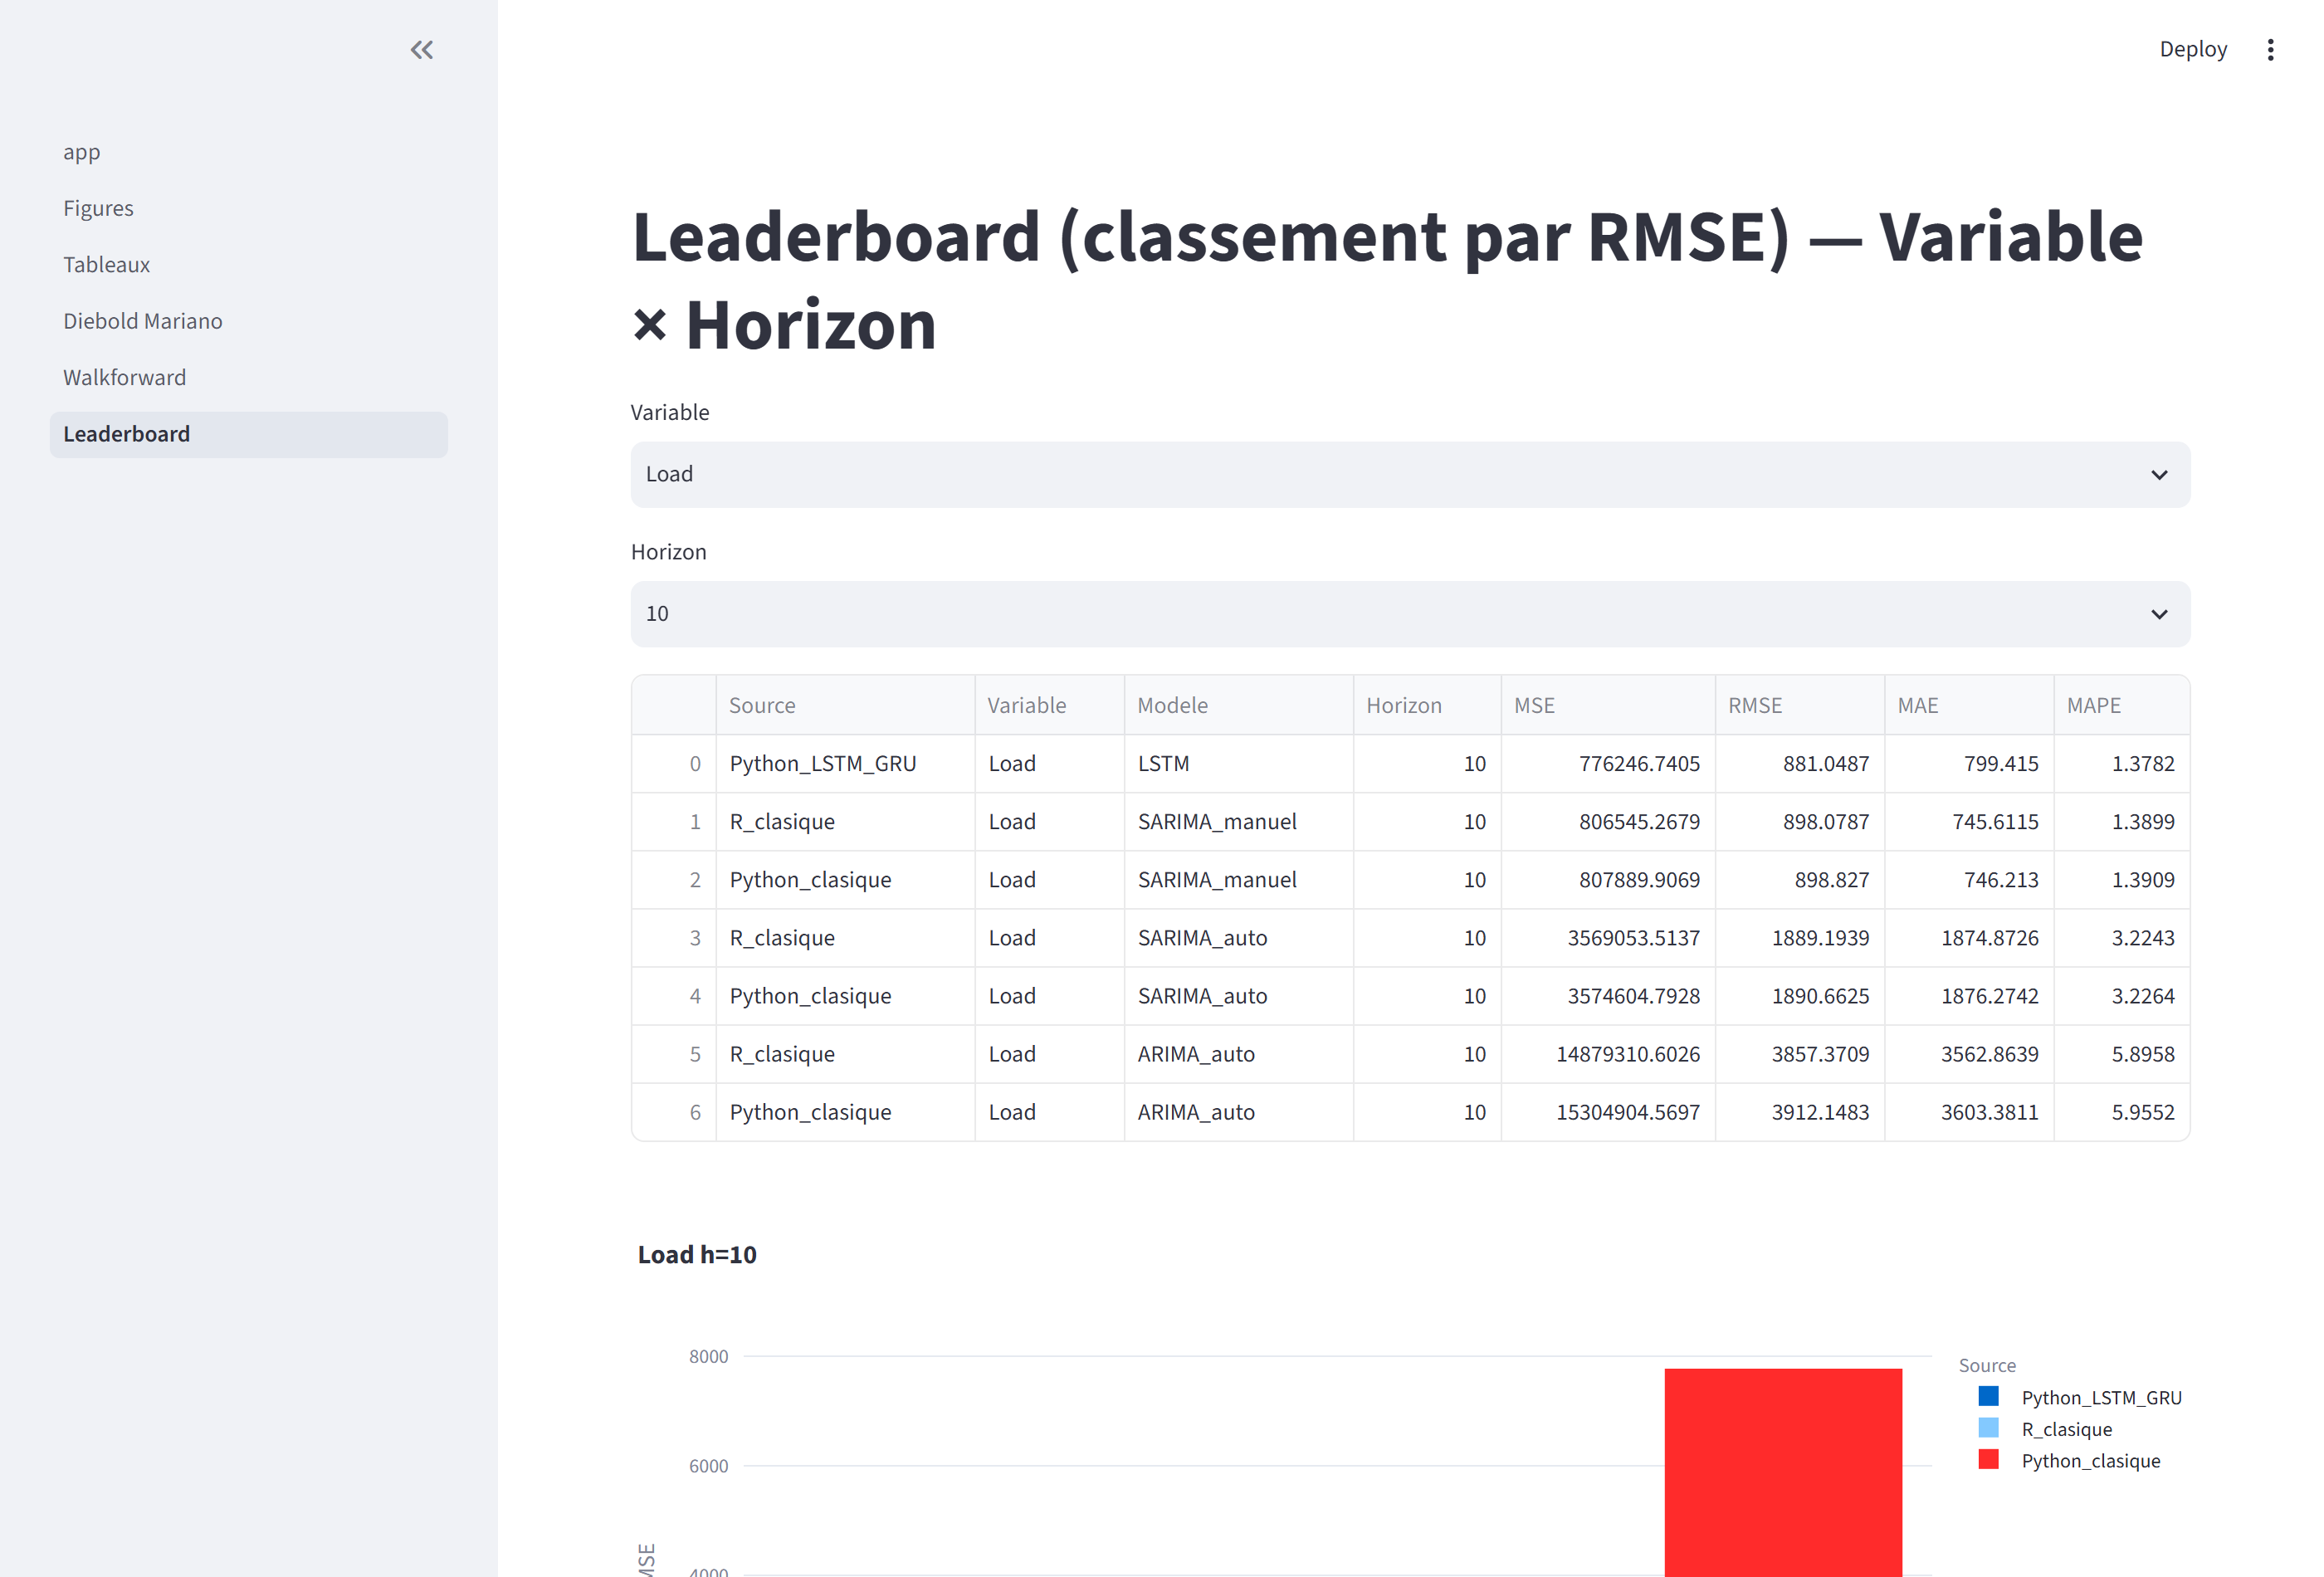
\includegraphics[width=0.9\textwidth]{dashboard_leaderboard.png}
\caption{Interface Streamlit --- leaderboard par variable et horizon.}
\label{fig:dash_leaderboard}
\end{figure}

\FloatBarrier
